\documentclass{beamer}
\usepackage[OT1]{fontenc}
\usepackage[utf8]{inputenc}
%\setmainfont{STIX}
%\usepackage{unicode-math}
%\setmathfont{STIX Math}

\usepackage[british]{babel}

\usepackage[export]{adjustbox}

\title{Biotech Beer Brewing}
\subtitle{Or: How I Learned to Stop Worrying and Control the Lactobacilli}
\author{Dominik Schmidt, ETH Zürich\\Jakob Wittman, TU München}
\institute{Háskóli Íslands}
\date{\today}
\titlegraphic{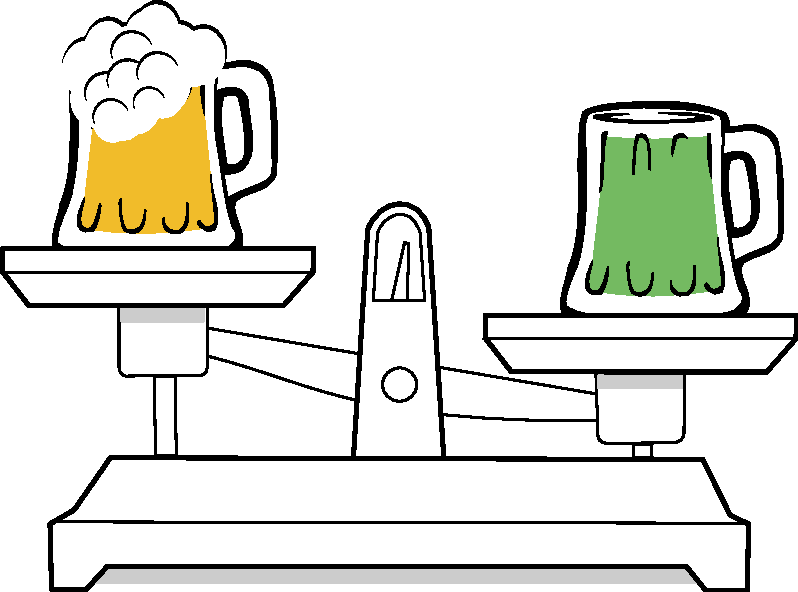
\includegraphics[width=0.3\linewidth]{../Graph/Logo.pdf}}
\logo{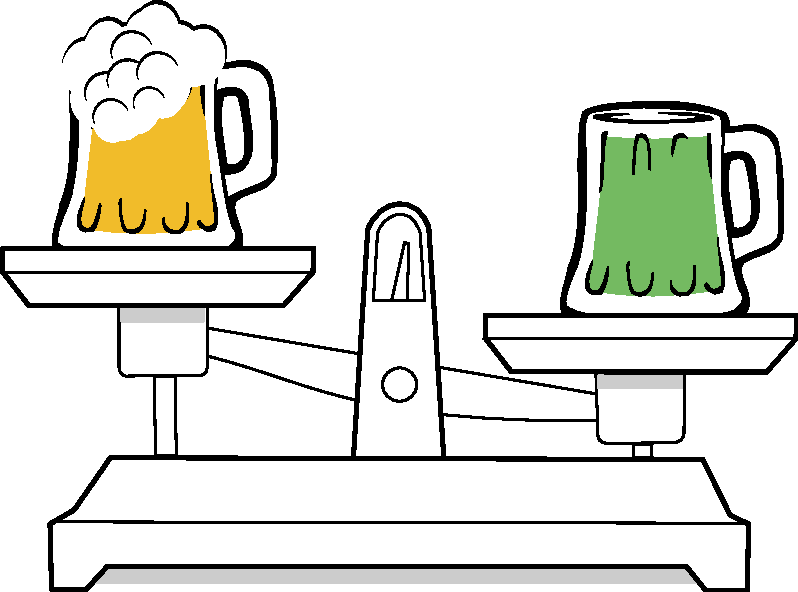
\includegraphics[width=5em]{../Graph/Logo.pdf}}
\beamertemplatenavigationsymbolsempty

\usepackage{xcolor}
\usepackage{tikz}
\usetikzlibrary{calc}
\usetikzlibrary{arrows}
\usetikzlibrary{positioning}

\begin{document}
\begin{frame}[plain]
	\begin{center}
	Silly Logos?\\[1.5em]
	Hold my...
	\end{center}
\end{frame}
%\begin{frame}[plain]
%	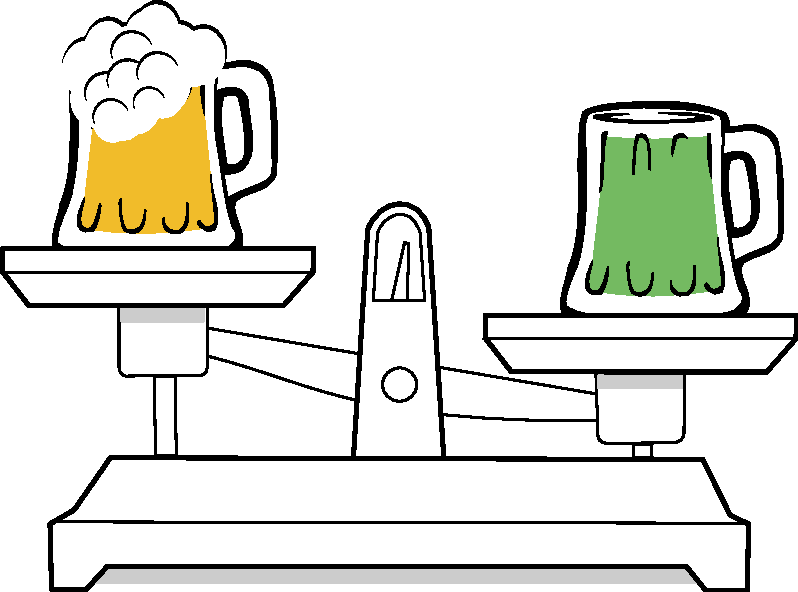
\includegraphics[width=\linewidth]{../Graph/Logo.pdf}
%\end{frame}
\begin{frame}[plain]
	\titlepage
\end{frame}
\section{What}
	\begin{frame}{What?!}
		\begin{minipage}{0.45\linewidth}
		\begin{itemize}
			\item Analyse coexistance of:
			\begin{itemize}
				\item Saccharomyces cerevisiae
				\item Lactobacillus Brevis
			\end{itemize}
			\item Understand how beer can turn sour
			\item See how sour beer can be prevented
		\end{itemize}
		\end{minipage}
		\begin{minipage}{0.45\linewidth}
		\centering
		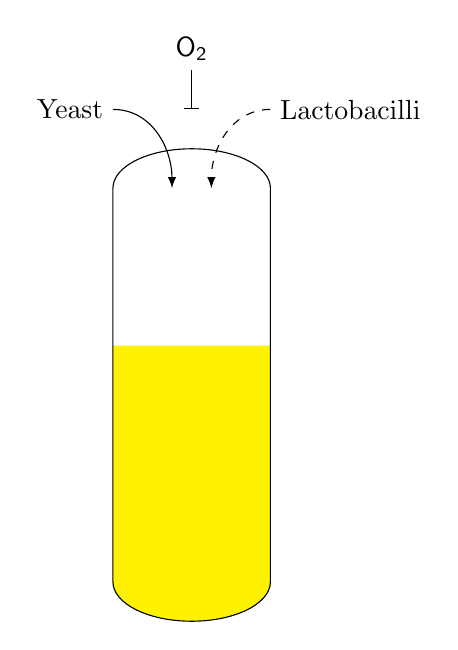
\begin{tikzpicture}
			\node[left] at(0, 6) (yeast){Yeast};
			\node[right] at(2, 6) (la){Lactobacilli};
			\node[above] at(1, 6.5) (ox){$\mathsf{O_2}$};
			\fill[fill=yellow] (0,0) -- (0,3) -- (2,3) -- (2,0) arc(0:-180:1 and 0.5);
			\draw (0,0) -- (0,5) arc(180:0:1 and 0.5) -- (2,0) arc(0:-180:1 and 0.5);
			\draw[-latex] (yeast.east) .. controls +(right:0.5) and +(up:0.5) .. (0.75,5);
			\draw[-latex, dashed] (la.west) .. controls +(left:0.5) and +(up:0.5) .. (1.25,5);
			\draw[-|] (ox.south) -- (1,6);
		\end{tikzpicture}
		\end{minipage}
	\end{frame}
\section{How}
	\begin{frame}{How?}
		\begin{itemize}
			\item Find beer-like initial conditions of medium
			\item Metabolite density via intake upper bounds
			\item Simulate population dynamics via $\mathsf{V_{Bio}}$
			\item Simluate metabolite flow and update the medium concentrations
			\item Homogeneity of medium is assumed
		\end{itemize}
		\begin{center}
		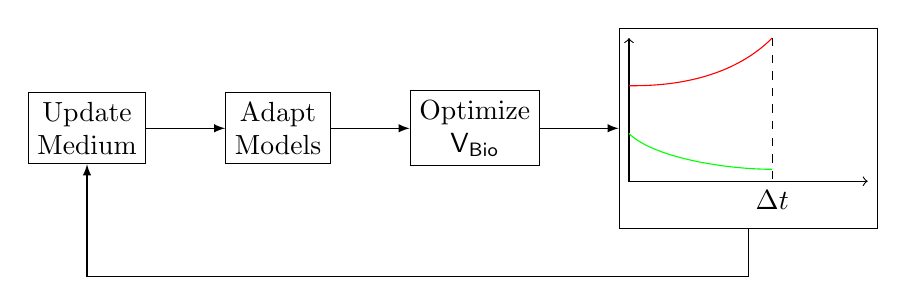
\begin{tikzpicture}[x=0.1\linewidth,y=0.1\linewidth]
			\tikzset{box/.style={shape=rectangle, draw=black,align=center}}
			\tikzset{flow/.style={-latex}}
			\node[box] (medium){Update\\Medium};
			\node[box, right=of medium] (bounds){Adapt\\Models};
			\node[box, right=of bounds](opt){Optimize\\$\mathsf{V_{Bio}}$};
			\node[box, right=of opt](sim){\tikz[scale=0.5]{\draw[<->](0,3) -- (0,0) -- (5,0); \draw[red] (0,2) .. controls (0.5,2) and (2,2) .. (3,3);\draw[green] (0,1) .. controls (0.5,0.5) and (2,0.25) .. (3,0.25); \draw[dashed] (3,3) -- (3,0) node[below]{$\Delta t$};}};
			\draw[flow] (medium.east) -- (bounds.west);
			\draw[flow] (bounds.east) -- (opt.west);
			\draw[flow] (opt.east) -- (sim.west);
			\draw[flow] (sim.south) -- +(down:0.5) -| (medium.south);
		\end{tikzpicture}
		\end{center}
	\end{frame}
\section{Why}
	\begin{frame}{Why}
		\begin{itemize}
			\item Find conditions favourable for good beer
			\item Level up our brewing skills 
			\item Help small-scale and craft breweries
			\item Potentially reduce desinfectant use in the industry
		\end{itemize}
		\begin{figure}
			\centering
			
\includegraphics[width=0.3\linewidth]{Img/AMIV_Braeu.pdf}
		\end{figure}
	\end{frame}
\end{document}
